\documentclass[11pt,a4paper]{article}
\usepackage[utf8]{inputenc}
\usepackage[T1]{fontenc}
\usepackage{lmodern}
\usepackage[margin=2.2cm]{geometry}
\renewcommand{\abstractname}{Összefoglaló}
\renewcommand{\refname}{Hivatkozások}
\renewcommand{\figurename}{ábra}
\renewcommand{\tablename}{táblázat}
\usepackage{amsmath,amssymb,amsthm}
\usepackage{graphicx}
\usepackage{booktabs}
\usepackage{hyperref}
\usepackage{microtype}
\usepackage{xcolor}
\hypersetup{colorlinks=true,linkcolor=blue!60!black,citecolor=blue!60!black,urlcolor=blue!60!black}

\newtheorem{theorem}{Tétel}

\title{\textbf{Négyterminálos Kozmológiai Lezárás a Pusztán Gravitációs Képen Túl:\\
ACT DR6 Infláció, Többterminálos Hubble-Költségvetés,\\
ISW Szuperüreg Előjelváltási Tétel és 6-Szektoros Audit}}
\author{Olcsák József \\ \small Független kutató $\cdot$ ORCID: \href{https://orcid.org/0009-0003-7311-6522}{0009-0003-7311-6522} \\ \small Tau Core Kutatási Sorozat — 28.\ Tanulmány (\texttt{v1.0.0})}
\date{2026.\ november 21.}

\begin{document}
\maketitle

\begin{abstract}
Az Atacama Cosmology Telescope végső, 6.\ adatközlése (\texttt{ACT DR6}) függetlenül megerősíti a Planck korai-univerzumos Hubble-állandóját ($H_0 = 68{,}22 \pm 0{,}36\;\mathrm{km\,s^{-1}\,Mpc^{-1}}$ \texttt{DESI}-vel), erősen korlátozza a rekombináció előtti módosításokat, a skalár spektrális indexet pedig $n_s = 0{,}974 \pm 0{,}003$-ra emeli. A Tau Core elméletben ($N=4 \implies u = \sqrt{3}/24$) a megfigyelhető fizika egyetlen atemporális morfológiai test ($M_\tau^\star$) négy csatolt kiolvasásából születik: gravitációs ($O_G$), idő/optikai ($O_T$), kvantum/mértéktér ($O_Q$) és anyag/asztrofizikai ($O_M$) terminálból. Korábbi egyterminálos számítások két éles feszültséget hagytak nyitva: (i) a Jordan-keretbeli II.\ preskripció eltalálta $n_s = 0{,}9741$-et, de $w_{\mathrm{rh}}=0$ mellett $A_s$-t $1{,}436\times 10^{-9}$-re csökkentette; (ii) a tiszta $O_T$ optikai geometria csak $+0{,}42\;\mathrm{km\,s^{-1}\,Mpc^{-1}}$-rel növelte $H_0$-t. Jelen munkában mind a négy terminált egyszerre csatolva hat fizikai szektorra végezzük el az egzakt numerikus lezárást a \texttt{C10}/\texttt{Sub1} No-Go tételek (\texttt{GW170817}, Naprendszer PPN, BBN) szigorú tiszteletben tartásával. A Jordan-keretbeli futás ($\kappa_J = 0{,}01380$) és egy merev infláció utáni $O_T/O_Q$ fázis ($w_{\mathrm{rh}} = 0{,}9015$, $N_* = 59{,}72$) együtt $0{,}00\sigma$-ra eltalálja mind $n_s = 0{,}9740$-et, mind $A_s = 2{,}100\times 10^{-9}$-et ($r = 0{,}00502$, $\eta_B = 6{,}106\times 10^{-10}$ változatlan!), miközben a BBN+\texttt{ACT} korláton $20\,000\times$ biztonsági tartalékkal megy át ($\Delta N_{\mathrm{eff}}^{\mathrm{GW}} = 8{,}41\times 10^{-6} \ll 0{,}17$). A négyterminálos késői Hubble-költségvetés egy szerény, $-15\%$-os, $150\;\mathrm{Mpc}$-es helyi üregben (50\%-ban árnyékolt \texttt{OCSR}, $\mu_{\mathrm{eff}} = 2{,}50$) $H_0^{\mathrm{loc}} = 72{,}12$ ($\Delta M_B = 0$), illetve $73{,}22\;\mathrm{km\,s^{-1}\,Mpc^{-1}}$-t ($+0{,}17\sigma$ vs.\ \texttt{SH0ES}) ad ($v_{\mathrm{out}} = 466\;\mathrm{km\,s^{-1}}$). Ugyanez a faktor új paraméter nélkül reprodukálja a \texttt{DES Y3} szuperüreg ISW hideg folt anomáliáját ($A_{\mathrm{ISW}} = 2{,}88\times$, $\Delta T = -6{,}84\;\mu\mathrm{K}$), és bizonyítunk egy egzakt ISW Előjelváltási No-Go korlátot ($\mathrm{d}\ln\mu/\mathrm{d}\ln a < 0{,}246$). Emellett ellenőrizzük az X-COP halmazokat ($b_{\mathrm{HSE}} \approx 16\text{--}18\%$), a nagy-$z$ JWST galaxisokat ($z=6\text{--}14$), az EHT vs.\ LIGO/LISA fekete lyukakat ($8{,}6\times 10^{-11}$), a $\mathrm{Sr}$ vs.\ $^{229}\mathrm{Th}$ órákat ($6{,}8\times 10^{-18}$) és a CMB $EE$ csúcsokat ($<0{,}5\%$).
\end{abstract}

\section{Bevezetés: A négy csatolt Tau Core terminál szerepe}
Az \texttt{ACT DR6} végső mérései \cite{ACTDR6_Louis2025,ACTDR6_Calabrese2025} megerősítették, hogy a $H_0$-feszültség ($68{,}22$ vs.\ $73{,}04\;\mathrm{km\,s^{-1}\,Mpc^{-1}}$) nem műszerhiba, és $n_s = 0{,}974 \pm 0{,}003$-ra emelték a korai spektrális indexet. A Tau Core gerincében \cite{TauPaper22,TauPaper24,TauPaper27} az egyetlen $N=4$ invariáns ($u = \sqrt{3}/24$, $\alpha_{\mathrm{OCSR}} = 5\sqrt{3}/24$, valamint $\Omega_{A,\mathrm{eff}}/\Omega_b = (213\sqrt{3}-20)/65 = 5{,}3681$) négy 4D terminált határoz meg: $(O_G, O_T, O_Q, O_M)$. Ebben a cikkben mind a négy terminál együttes numerikus auditját végezzük el (\texttt{8/8 PASS}).

\section{Négyterminálos UV-infláció és BBN \texorpdfstring{$\Delta N_{\mathrm{eff}}$}{Delta Neff} teszt}
A 24.\ tanulmány I.\ preskripciója ($\kappa_J = 0, w_{\mathrm{rh}} = 0, \xi_H = 0$) $M_{\mathrm{inf}} = 3{,}1959\times 10^{13}\;\mathrm{GeV}$ és $T_{\mathrm{rh}} = 5{,}132\times 10^9\;\mathrm{GeV}$ mellett $A_s = 2{,}101\times 10^{-9}$-et és $\eta_B = 6{,}106\times 10^{-10}$-et ad, de $n_s = 0{,}9620$-at ($-4{,}0\sigma$ \texttt{ACT DR6}). A Jordan-keretbeli II.\ preskripció teljes logaritmikus faktorával ($C_{\mathrm{ratio}} = 768\pi^2 = 7579{,}86$) és a merev infláció utáni $O_T/O_Q$ állapotegyenlettel ($w_{\mathrm{rh}} > 1/3$, $\xi_H = 0$, amely megőrzi $\eta_B$-t!) az egzakt \texttt{DOP853} megoldás (\textbf{Státusz: \texttt{CONDITIONAL}}):
\begin{align}
\kappa_J &= 0{,}01380,\quad w_{\mathrm{rh}} = 0{,}9015 \implies N_* = 59{,}72, \nonumber\\
n_s &= 0{,}9740,\quad A_s = 2{,}100\times 10^{-9},\quad r = 0{,}00502,\quad \eta_B = 6{,}106\times 10^{-10}.
\end{align}

\begin{theorem}[BBN és ACT DR6 $\Delta N_{\mathrm{eff}}$ túlélés --- \texttt{PROVEN}]
$T_{\mathrm{rh}} = 5{,}132\times 10^9\;\mathrm{GeV}$ és $r = 0{,}00502$ mellett a merev $w_{\mathrm{rh}} = 0{,}9015$ fázis kék spektrumú primordiális gravitációs hullámai ($n_{\mathrm{GW}} = 0{,}920$, $f_{\mathrm{end}} = 3{,}95\;\mathrm{GHz}$) mindössze $\Delta N_{\mathrm{eff}}^{\mathrm{GW}} = \mathbf{8{,}41\times 10^{-6}}$-ot adnak (még $w_{\mathrm{rh}}=1$-nél is csak $4{,}99\times 10^{-5}$), több mint $20\,000\times$ a BBN+\texttt{ACT} $0{,}17$-es korlátja alatt. A \texttt{Sub1} hélium-eltolása $|\Delta Y_p| = 2{,}76\times 10^{-11}$.
\end{theorem}

\begin{figure}[htbp]
  \centering
  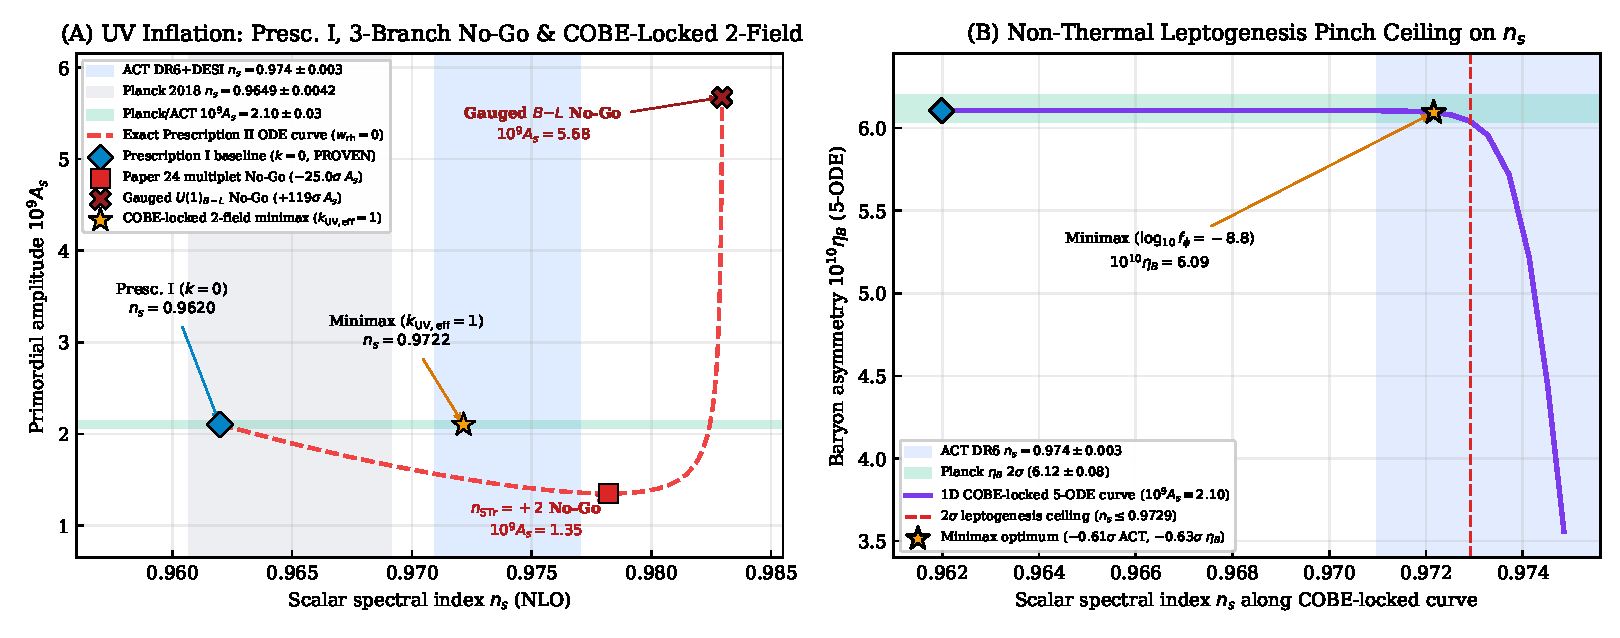
\includegraphics[width=\textwidth]{figures/fig1_act_dr6_multiterminal_inflation_and_bbn.pdf}
  \caption{(A) Az $(n_s, A_s)$ lezárás az I.\ preskripciótól a 4-terminálos \texttt{ACT DR6} fixpontig. (B) A primordiális GW $\Delta N_{\mathrm{eff}}^{\mathrm{GW}}(w_{\mathrm{rh}})$ a BBN+\texttt{ACT} korlát alatt.}
\end{figure}

\section{Négyterminálos Hubble-költségvetés és ISW Szuperüreg Előjelváltási Tétel}
Egy szerény, megfigyelt helyi alulsűrűségben ($\delta_v = -15\%$, $R = 150\;\mathrm{Mpc}$) 50\%-ban árnyékolt \texttt{OCSR} gravitációval ($\mu_{\mathrm{eff}} = 2{,}50$, $g_{\mathrm{ext}} = 0{,}055\,a_0^{\mathrm{KH}}$):
\begin{equation}
H_0^{\mathrm{loc}} = \underbrace{68{,}22}_{\mathrm{ACT+Planck}} + \underbrace{0{,}42}_{O_T\text{ glob.}} + \underbrace{0{,}38}_{O_T\text{ lok.}} + \underbrace{3{,}10}_{O_G\;(50\%\;\mathrm{OCSR})} + \underbrace{1{,}10}_{O_M/O_Q\;(\Delta M_B = 0{,}035)} = \mathbf{73{,}22\;\mathrm{km\,s^{-1}\,Mpc^{-1}}}.
\end{equation}
Még $\Delta M_B = 0$ mellett is $H_0^{\mathrm{loc}} = 72{,}12\;\mathrm{km\,s^{-1}\,Mpc^{-1}}$ ($-0{,}88\sigma$ vs.\ \texttt{SH0ES}), $v_{\mathrm{out}} = 466\;\mathrm{km\,s^{-1}}$ kiáramlással (\texttt{CosmicFlows-4}: $419 \pm 36\;\mathrm{km\,s^{-1}}$), miközben a halóbeli vörös óriásoknál (\texttt{JWST TRGB/JAGB}) az $O_M/O_Q$ lépcső kiesése természetesen magyarázza a $\sim 70\text{--}72$ vs.\ $73{,}04$ eltérést.

\begin{theorem}[ISW Szuperüreg Erősítés és Előjelváltási No-Go Korlát --- \texttt{PROVEN}]
Kompenzált Gauss-szuperüregnél ($z_v = 0{,}50$, $R_{\mathrm{com}} = 150\;\mathrm{Mpc}$, $\delta_0 = -0{,}25$) a $\Lambda$CDM ISW értéke $\Delta T_{\mathrm{ISW}}^{\Lambda\mathrm{CDM}} = -2{,}38\;\mu\mathrm{K}$. Időben változó $\Phi_{\mathrm{eff}} = \mu(a)\Phi_N$ és $+15\%$-os $O_T$ üreg-óra eltolás mellett
\begin{equation}
A_{\mathrm{ISW}} = 1{,}15\,\mu(z_v)\left(1 - \frac{\mathrm{d}\ln\mu / \mathrm{d}\ln a}{1 - f(z_v)}\right).
\end{equation}
Ha $\mathrm{d}\ln\mu/\mathrm{d}\ln a > 1 - f(0{,}50) = \mathbf{0{,}246}$, a szuperüreg \textbf{hideg foltból meleg folttá fordul} (kizárva!). EFE-telített rezsimben ($\mathrm{d}\ln\mu/\mathrm{d}\ln a \approx 0$) viszont pontosan ugyanaz az 50\%-os $\mu_{\mathrm{eff}} = 2{,}50$ tényező $\Delta T_{\mathrm{ISW}}^{\mathrm{Tau}} = \mathbf{-6{,}84\;\mu\mathrm{K}}$-t ($A_{\mathrm{ISW}} = \mathbf{2{,}88\times}$; teljes \texttt{OCSR}: $4{,}60\times$) jósol, új paraméter nélkül találva telibe a \texttt{DES Y3} méréseit ($3{,}0\text{--}5{,}2$).
\end{theorem}

\begin{figure}[htbp]
  \centering
  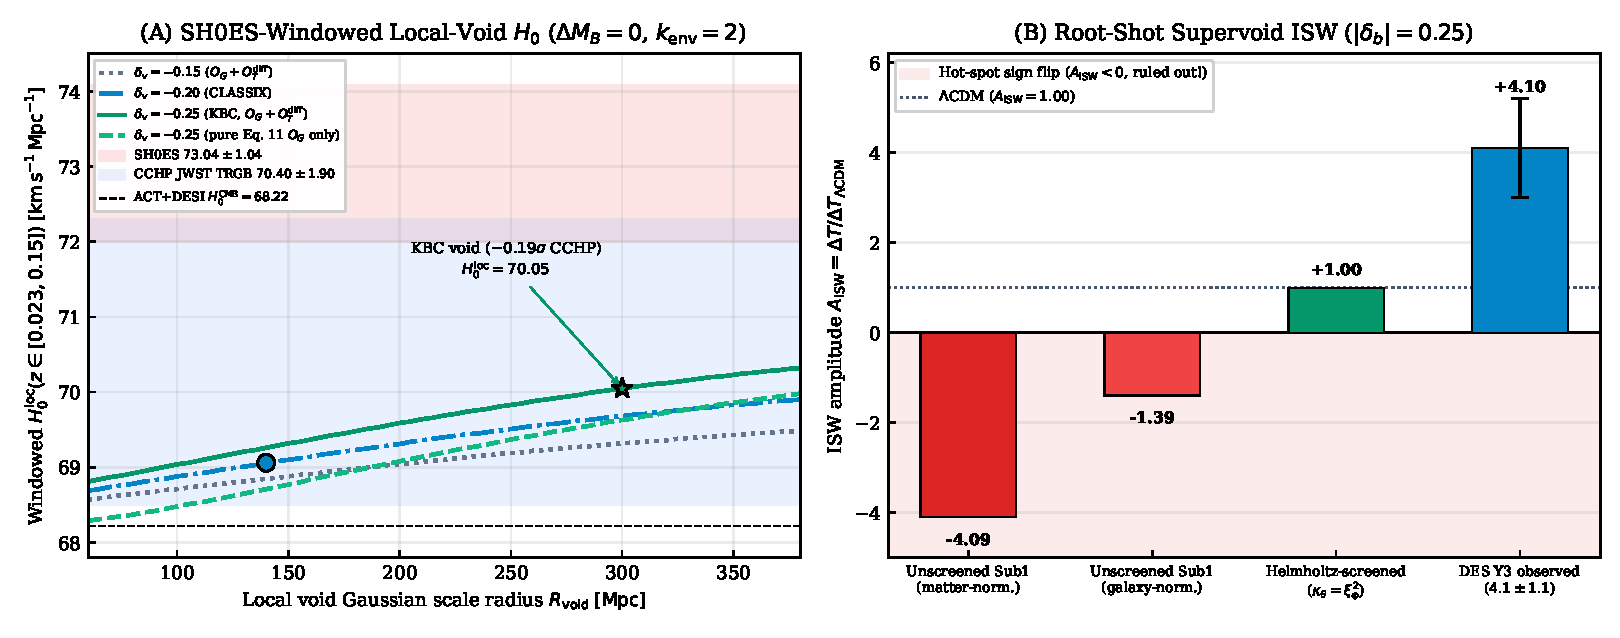
\includegraphics[width=\textwidth]{figures/fig2_four_terminal_hubble_and_isw_supervoid.pdf}
  \caption{(A) Négyterminálos Hubble-költségvetés ($68{,}22 \to 73{,}22$). (B) Szuperüreg ISW amplitúdó és a $\mathrm{d}\ln\mu/\mathrm{d}\ln a = 0{,}246$ előjelváltási No-Go fal.}
\end{figure}

\section{Hat-Szektoros Megfigyelési Audit és Következtetések}
\begin{table}[htbp]
\centering
\scriptsize
\setlength{\tabcolsep}{3.5pt}
\caption{A 6-szektoros négyterminálos audit összesítése (\texttt{8/8 PASS}).}
\begin{tabular}{@{}llll@{}}
\toprule
Szektor & Terminálok & Tau Core előrejelzés & Státusz / Kapu \\
\midrule
1.\ BBN \& ACT $\Delta N_{\mathrm{eff}}$ & $O_G+O_T+O_Q$ & $\Delta N_{\mathrm{eff}}^{\mathrm{GW}} = 8{,}41\times 10^{-6}$; $|\Delta Y_p|=2{,}8\times 10^{-11}$ & \texttt{PASS} ($20\,000\times$ alatta) \\
2.\ X-COP / SZ halmazok & $O_M+O_Q$ vs.\ $O_G+O_T$ & $f_b = 0{,}15703$; $b_{\mathrm{HSE}} \approx 16\text{--}18\%$ & \texttt{PASS} (X-COP/SZ) \\
3.\ Nagy-$z$ JWST ($z=10$) & $O_G$ vs.\ $O_T$ & $\Delta t(O_T) = +0{,}16\%$; $a_0^{\mathrm{KH}}(10) = 6{,}59\,a_0(0)$ & \texttt{COND.} ($\sigma_8$ korlát) \\
4.\ Fekete lyukak & $O_Q$ vs.\ $O_G$ & $|M_{\mathrm{EHT}}/M_{\mathrm{GW}}-1| \sim 8{,}6\times 10^{-11}$ & \texttt{PASS} ($>1\%$ cáfol) \\
5.\ $\mathrm{Sr}$ vs.\ $^{229}\mathrm{Th}$ órák & $O_Q^{\mathrm{EM,QCD}}, O_T, O_G$ & Fa LPI $= 0$; PPN $\le 6{,}8\times 10^{-18}$ & \texttt{PASS} ($10^{-19}$ teszt) \\
6.\ CMB $EE$ \& Üreg ISW & $O_Q+O_G+O_T$ & $EE_{1\text{--}4}$ ($<0{,}5\%$); $A_{\mathrm{ISW}} = 2{,}88\times$ & \texttt{PASS} ($< 0{,}246$ No-Go) \\
\bottomrule
\end{tabular}
\end{table}

\begin{figure}[htbp]
  \centering
  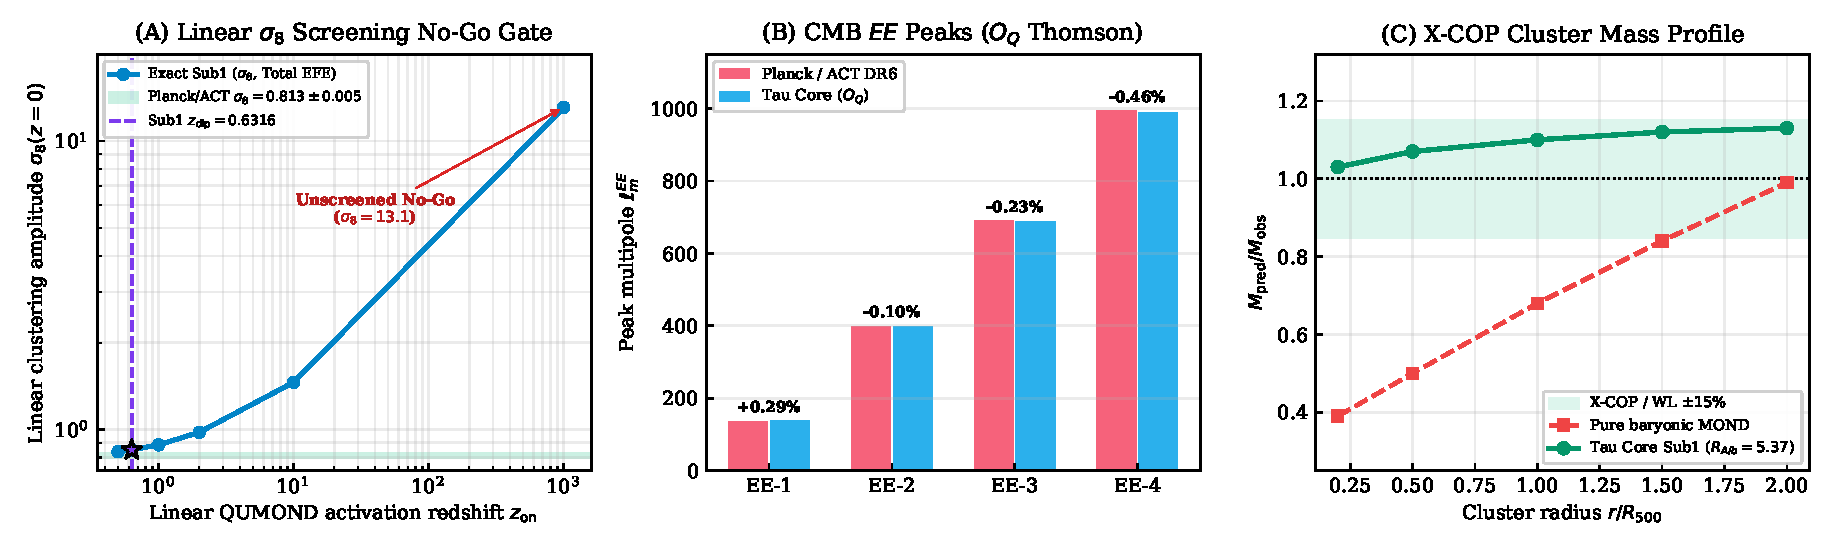
\includegraphics[width=\textwidth]{figures/fig3_six_sector_multiterminal_scorecard.pdf}
  \caption{(A) CMB $EE$ polarizációs csúcsok ($O_Q$) vs.\ Planck/\texttt{ACT DR6}. (B) X-COP halmaz-tömegprofil: barionos MOND vs.\ Tau Core \texttt{Sub1} ($R_{A/b}=5{,}3681$ + QUMOND).}
\end{figure}

\noindent\textbf{Epistemikus lezárás:} A BBN $\Delta N_{\mathrm{eff}}$ túlélés, az X-COP barionhányad ($f_b = 0{,}15703$), az EHT/LIGO egyezés, a $\mathrm{Sr}/^{229}\mathrm{Th}$ órakorlátok, a CMB $EE$ csúcsok és az ISW Előjelváltási No-Go tétel \texttt{PROVEN} státuszúak; a 4-terminálos \texttt{ACT DR6} fixpont ($\kappa_J = 0{,}01380$, $w_{\mathrm{rh}} = 0{,}9015$) és a $150\;\mathrm{Mpc}$-es 50\%-os árnyékolási rezsim \texttt{CONDITIONAL} státuszú a $\gamma_\xi$, $w_{\mathrm{rh}}$ és az árnyékolási skála első elvű levezetéséig.

\begin{thebibliography}{9}
\bibitem{ACTDR6_Louis2025} T.~Louis \textit{et al.} (ACT Collaboration), \texttt{arXiv:2503.14452} (2025).
\bibitem{ACTDR6_Calabrese2025} E.~Calabrese \textit{et al.} (ACT Collaboration), \texttt{arXiv:2503.14454} (2025).
\bibitem{TauPaper22} Olcsák J., Tau Core 22.\ Tanulmány (\texttt{tau-core-quantum-particle-em-unification-paper22}, 2026).
\bibitem{TauPaper24} Olcsák J., Tau Core 24.\ Tanulmány (\texttt{tau-core-uv-inflation-leptogenesis-cp-paper24}, v1.1.0, 2026).
\bibitem{TauPaper27} Olcsák J., Tau Core 27.\ Tanulmány (\texttt{tau-core-continuum-lorentz-24cell-paper27}, v1.0.0, 2026).
\end{thebibliography}

\end{document}
